%Do not alter this block of commands.  If you're proficient at LaTeX, you may include additional packages, create macros, etc. immediately below this block of commands, but make sure to NOT alter the header, margin, and comment settings here. 
\documentclass[12pt]{article}
 \usepackage[margin=1in, bottom=4.5cm]{geometry}
\usepackage{amsmath,amsthm,amssymb,amsfonts, enumitem, fancyhdr, color, comment, graphicx, environ, scrextend}
\usepackage[table,dvipsnames]{xcolor}
\usepackage{tikz}  
\usepackage{tikz-3dplot} 
\usepackage{amssymb}
\usepackage{xifthen}
\pagestyle{fancy}
\setlength{\headheight}{65pt}
\newenvironment{problem}[2][Problem]{\begin{trivlist}
\item[\hskip \labelsep {\bfseries #1}\hskip \labelsep {\bfseries #2.}]}{\end{trivlist}}
\newenvironment{sol}
    {\emph{Proof.}
    }
    {
    \qed
    }
\specialcomment{com}{ \color{blue} \textbf{Comment:} }{\color{black}} %for instructor comments while grading
\NewEnviron{probscore}{\marginpar{ \color{blue} \tiny Problem Score: \BODY \color{black} }}
%%%%%%%%%%%%%%%%%%%%%%%%%%%%%%%%%%%%%%%%%%%%%%%%%%%%%%%%%%%%%%%%%%%%%%%%%%%%%%%%%

\newcommand\restr[2]{{% we make the whole thing an ordinary symbol
  \left.\kern-\nulldelimiterspace % automatically resize the bar with \right
  #1 % the function
  \vphantom{\big|} % pretend it's a little taller at normal size
  \right|_{#2} % this is the delimiter
  }}





%%%%%%%%%%%%%%%%%%%%%%%%%%%%%%%%%%%%%%%%%%%%%
%Fill in the appropriate information below
\lhead{Trey Manuszak}  %replace with your name
\rhead{MAT 473: Intermediate Real Analysis II \\ Homework 6: 21, 22, 23, 24} %replace XYZ with the homework course number, semester (e.g. ``Spring 2019"), and assignment number.
%%%%%%%%%%%%%%%%%%%%%%%%%%%%%%%%%%%%%%%%%%%%%

\usepackage{blindtext}
\title{MAT 473: Intermediate Real Analysis II}
\date{February 27, 2020}
\author{Trey Manuszak\\ Arizona State University}



%%%%%%%%%%%%%%%%%%%%%%%%%%%%%%%%%%%%%%
%Do not alter this block.
\begin{document}
%%%%%%%%%%%%%%%%%%%%%%%%%%%%%%%%%%%%%%




\maketitle
\newpage



%Solutions to problems go below.  Please follow the guidelines from https://www.overleaf.com/read/sfbcjxcgsnsk/


%Copy the following block of text for each problem in the assignment.
Problems 21 - 22 finish the proof of the implicit function theorem in two variables. Let $f : U \subseteq \mathbb{R}^2 \to \mathbb{R}$, $(a,b) \in U$, $c = f(a,b)$, and $g : (a-s,a+s) \to (b-r,b+r)$ be as in the implicit function theorem (Theorem 9.1 in the notes). It has been shown that $g$ is continuous on $(a-s, a+s)$. Complete the proof of the theorem by showing that $g$ is differentiable on $(a-s,a+s)$, with derivative $g'(x) = -D_1f(x,g(x))/D_2f(x,g(x))$, using the following outline.

\begin{problem}{21}
First prove it for $x = a$ as follows. Let $A = D_1f(a,b)$ and $B = D_2f(a,b)$ (so that $f'(a,b)$ has a matrix $(A \hspace{.5em} B) \in M_{1 \times 2}$.) Let $x \in (a-s,a+s)$ and set $h = x-a,k = g(x)-b$.

\begin{itemize}
    \item[(a)] Prove that there are real-valued functions $\psi_1$ and $\psi_2$ defined in a neighborhood of 0 such that $\lim_{(x,y)\to 0}\phi_i(x,y) = 0$ for $i = 1,2$, and such that $$\frac{h}{k} + \frac{A}{B} + \frac{1}{B}\psi_1(h,k) + \frac{1}{B}\psi_2(h,k)\frac{k}{h} = 0.$$ (Hint: let $\phi(h,k)$ be as in the alternate version of differentiability of $f$ (notes, Lemma 3.16), and write $$\phi(h,k)\lVert (h,k) \rVert = \phi(h,k) \frac{\lVert (h,k) \rVert}{\left| h \right| + \left| k \right|} \left( \frac{\left| h \right|}{h}h + \frac{\left| k \right|}{k}k  \right).)$$
    
    \begin{sol}
    Let $f : U \subseteq \mathbb{R}^2 \to \mathbb{R}$ be continuously differentiable, let $(a,b) \in U$ with $D_2f(a,b) \neq 0$. Let $c = f(a,b)$. Let $g : B_s(a) \to B_r(b)$ with $f(x,,g(x)) = c$. Let $A = D_1f(a,b)$ and $B = D_2f(a,b)$. Now, there exists $\phi : B_r(0) \to \mathbb{R}$, since $f$ is differentiable, such that $\phi(0) = 0$, $\phi$ is continuous at 0, and $f(a+h) = f(a) + T(h) + \phi(h)\lVert h \rVert$. Define $\psi_1,\psi_2 : B_r(0) \to \mathbb{R}$ by $$\psi_1(h,k) = \begin{cases} 
      \frac{\phi(h,k) \lVert (h,k) \rVert \left| h \right|}{(\left| h \right| + \left| k \right| )h}, & \text{if } h \neq 0 \\
      0, & \text{if } h = 0
   \end{cases}$$
   and $$\psi_2(h,k) = \begin{cases} 
      \frac{\phi(h,k) \lVert (h,k) \rVert \left| k \right|}{(\left| h \right| + \left| k \right| )k}, & \text{if } k \neq 0 \\
      0, & \text{if } k = 0.
   \end{cases}$$
   
   \hspace{1em} Note, $\lim_{(h,k) \to 0}\phi(h,k) = 0$ because of the definition of $\phi$, which implies that \newline $\lim_{(h,k) \to 0}\psi_1(h,k) = 0$ and $\lim_{(h,k) \to 0}\psi_2(h,k) = 0$. Let $x \in (a-s,a+s) \setminus \{a\}$ such that $(x-a,g(x)-b) \in B_r(0)$. Let $h = x-a$ and $k = g(x) - b$. Therefore, by definition of $\phi$, $f((a,b)+(h,k)) = f(a,b) + f'(a,b)(h,k) + \phi(h,k) \lVert(h,k) \rVert$. So, $f((a,b) + (h,k)) = f((a,b) + (x-a,g(x)-b)) = f(x,g(x)) = c$ and $f(a,b) = c$, which gives us \begin{align*}
       0 &= f'(a,b)(h,k) + \phi(h,k) \lVert(h,k) \rVert \\
       &= (A \hspace{.5em} B)(h,k) + \phi(h,k)\frac{\lVert (h,k) \rVert}{\left| h \right| + \left| k \right|}\left( \frac{\left| h \right|}{h}h + \frac{\left| k \right|}{k}k \right) \\ 
       &= (A \hspace{.5em} B)(h,k) + \frac{\phi(h,k)\lVert (h,k) \rVert \left| h \right|}{(\left| h \right| + \left| k \right|)}\cdot h + \frac{\phi(h,k)\lVert (h,k) \rVert \left| k \right|}{(\left| h \right| + \left| k \right|)}\cdot k \\ 
       &= (A \hspace{.5em} B)(h,k) + \psi_1(h,k) \cdot h + \psi_2(h,k) \cdot k \tag*{(By definition of $\psi_1$ and $\psi_2$)} \\ 
       &= Ah + Bk + \psi_1(h,k) \cdot h + \psi_2(h,k) \cdot k \\ 
       &= Bh \left( \frac{A}{B} + \frac{k}{h} + \frac{1}{B}\psi_1(h,k) + \frac{1}{b}\psi_2(h,k)\frac{k}{h} \right) \\ 
       &= \frac{h}{k} + \frac{A}{B} + \frac{1}{B}\psi_1(h,k) + \frac{1}{B}\psi_2(h,k)\frac{k}{h}. \tag*{(Since $B = D_2f(a,b) \neq 0$)}
   \end{align*}
    \end{sol}
    
    \item[(b)] Prove that $g'(a) = -A/B.$ (Hint: solve for $\frac{h}{k}$ in part (a).)
    
    \begin{sol}
    Solving $\frac{h}{k} + \frac{A}{B} + \frac{1}{B}\psi_1(h,k) + \frac{1}{B}\psi_2(h,k)\frac{k}{h} = 0$ for $\frac{k}{h}$, then we get $$\frac{k}{h} = \frac{-(A + \psi_1(h,k))}{B + \psi_2(h,k)}.$$ Then, \begin{align*}
        \lim_{x \to a}\frac{g(a) - g(x)}{a-x} &= \lim_{x \to a}\frac{g(x) - g(a)}{x-a} \\ &= \lim_{x \to a}\frac{g(x) - b}{x-a} \\ &= \lim_{(h,k) \to 0} \frac{k}{h} \tag*{(By definition of $h$ and $k$)}\\ &= \frac{-(A + \psi_1(h,k))}{B + \psi_2(h,k)} \\ &= \frac{-A}{B}. \tag*{(Since $\lim_{(h,k) \to 0} \psi_{1,2} = 0$)}
    \end{align*}
    Therefore, $g'(a) = \frac{-A}{B}$.
    \end{sol}
\end{itemize}
\end{problem}


\begin{problem}{22}
Finish the proof of the implicit function theorem. Also show that if $f$ in the statement is $C^k$ for $k > 1$ the $g$ is also $C^k$.
\end{problem}

\begin{sol}
Continuing, we must show that $g$ is continuous at all $a \in B_s(a)$. Let $\epsilon > 0$ be arbitrary but fixed. Let $a' \in B_s(a)$ be arbitrary but fixed. Let $b' \in B_r(b)$ such that $g(a') = b'$. Let $Z = \{(x,y) \in \mathbb{R}^2 : x \in B_s(a),y \in B_r(b),\left|y - b'\right| < \epsilon\}$. Now, by construction of $s$, $D_2\restr{f}{Z}(a',b') \neq 0$. So, we now have a $B_s(a)',B_r(b)'$ such that $B_s(a)' \subseteq B_s(a)$ and $B_r(b)' \subseteq B_r(b)$ and $g_1$ such that $g_1 : B_s(a)' \to B_r(b)'$ such that for each $x \in B_s(a)$, $D_i(x,g_1(x)) = 0$ for $i = 1,2$ and $d(g_1(x),b') < \epsilon$. But, by uniqueness of $g(x)$, we get $g_1(x)$ for all $x \in B_s(a)$. Thus, for all $x \in B_s(a)$, $d(g(x),g_1(x)) < \epsilon$. Hence, $g$ is continuous at $a'$. But, since $a'$ was arbitrary in $B_s(a)$, then $g$ is continuous in over $B_s(a)$.  

Now, on showing $f$ is $C^k$ implies $g$ is $C^k$, we have already proven the base case of if $f$ is $C^1$, then $g$ is $C^1$. So, we will continue with the inductive step. Suppose the theorem is true for some $k > 1$. So, when $f$ is $C^{k+1}$, then $g$ is $C^k$. This is because $A,B^{-1} \in C^k$ and $g$ is a composition of the two. Therefore, $g' \in C^k$, which implies $g \in C^{k+1}$. Therefore, if $f$ is $C^k$, then $g$ is $C^k$.  
\end{sol}


\begin{problem}{23}
Let $f : \mathbb{R}^3 \to \mathbb{R}^2$ be given by $f(\rho, \phi, \theta) = (\rho\sin\phi\sin\theta,\rho\cos\phi)$.

\begin{itemize}
    \item[(a)] Use the implicit function theorem to show that the equation $f(\rho,\phi,\theta) = (1,1)$ can be solved for $(\phi,\theta)$ as a function of $\rho$ near the point $(\sqrt{3},\tan^{-1}\sqrt{2}, \pi/4)$.
    
    \begin{sol}
    Consider the surface $S := \{(\rho, \phi, \theta) \in \mathbb{R}^3 : \rho\sin\phi\sin\theta = 1 \text{ and } \rho\cos\phi = 1\}$. This can be rewritten as $\{(\rho, \phi, \theta) \in \mathbb{R}^3 : f(\rho, \phi, \theta) = (0,0)\}$ where $f : \mathbb{R}^3 \to \mathbb{R}^2$ is given by $f(\rho, \phi, \theta) := (\rho\sin\phi\sin\theta - 1,\rho\cos\phi - 1)$.
    %%%% 
    Then, \begin{align*}
        f'(\rho, \phi, \theta) &= \begin{pmatrix}
D_1f_1 & D_2f_1 & D_3f_1 \\ 
D_1f_2 & D_2f_2 & D_3f_2
\end{pmatrix} \\ &= \begin{pmatrix}
\sin\left(\phi\right) \sin\left(\theta\right) & \rho \cos\left(\phi\right) \sin\left(\theta\right) & \rho \cos\left(\theta\right) \sin\left(\phi\right) \\ 
\cos\left(\phi\right) & -\rho \sin\left(\phi\right) & 0
\end{pmatrix}.
    \end{align*}
    
    Now, at $(\sqrt{3},\tan^{-1}\sqrt{2}, \pi/4)$, we have $$f'(\sqrt{3},\tan^{-1}\sqrt{2}, \pi/4) = \begin{pmatrix}
\frac{\sqrt{3}}{3} & \frac{\sqrt{2}}{2} & 1 \\ 
\frac{\sqrt{3}}{3} & -\sqrt{2} & 0
\end{pmatrix}.$$ So, $\frac{\partial f}{\partial (\phi, \theta)}(\sqrt{3},\tan^{-1}\sqrt{2}, \pi/4) = \begin{pmatrix}
\frac{\sqrt{2}}{2} & 1 \\ 
-\sqrt{2} & 0
\end{pmatrix}$ and has a determinant $0+\sqrt{2} = \sqrt{2} \neq 0$. Since the matrix is invertible, then by the implicit function theorem, there exists $r,s > 0$, and a unique function $g : (\sqrt{3}-s,\sqrt{3}+s) \to B_r\left((\tan^{-1}\sqrt{2},\pi/4)\right)$, such that $f(\rho,g(\rho)) = (0,0)$ for all $x \in (\sqrt{3}-s,\sqrt{3}+s)$.
    \end{sol}
    
    \item[(b)] Use the implicit function theorem to find $\phi'(\sqrt{3})$ and $\theta'(\sqrt{3})$.
    
    \begin{sol}
    We have that $\frac{\partial f}{\partial \theta}(\sqrt{3},\tan^{-1}\sqrt{2}, \pi/4) = \begin{pmatrix} \frac{\sqrt{3}}{3} \\ \frac{\sqrt{3}}{3} \end{pmatrix}$. So, \begin{align*}
        g'(\sqrt{3}) &= -\begin{pmatrix}
\frac{\sqrt{2}}{2} & 1 \\ 
-\sqrt{2} & 0
\end{pmatrix}^{-1} \begin{pmatrix} \frac{\sqrt{3}}{3} \\ \frac{\sqrt{3}}{3} \end{pmatrix} \\ &= -\left( \frac{1}{2} \right)\begin{pmatrix}
0 & -\sqrt{2} \\ 
2 & 1
\end{pmatrix}\begin{pmatrix} \frac{\sqrt{3}}{3} \\ \frac{\sqrt{3}}{3} \end{pmatrix} \\ &= \begin{pmatrix} \frac{\sqrt{6}}{6} \\ -\frac{\sqrt{3}}{2} \end{pmatrix}.
    \end{align*}
    Therefore, $\phi'(\sqrt{3}) = \frac{\sqrt{6}}{6}$ and $\theta'(\sqrt{3}) = -\frac{\sqrt{3}}{2}$.
    \end{sol}
    
    \item[(c)] Give a geometric description of the situation, and explain why the results are reasonable.
    
    \begin{center}
    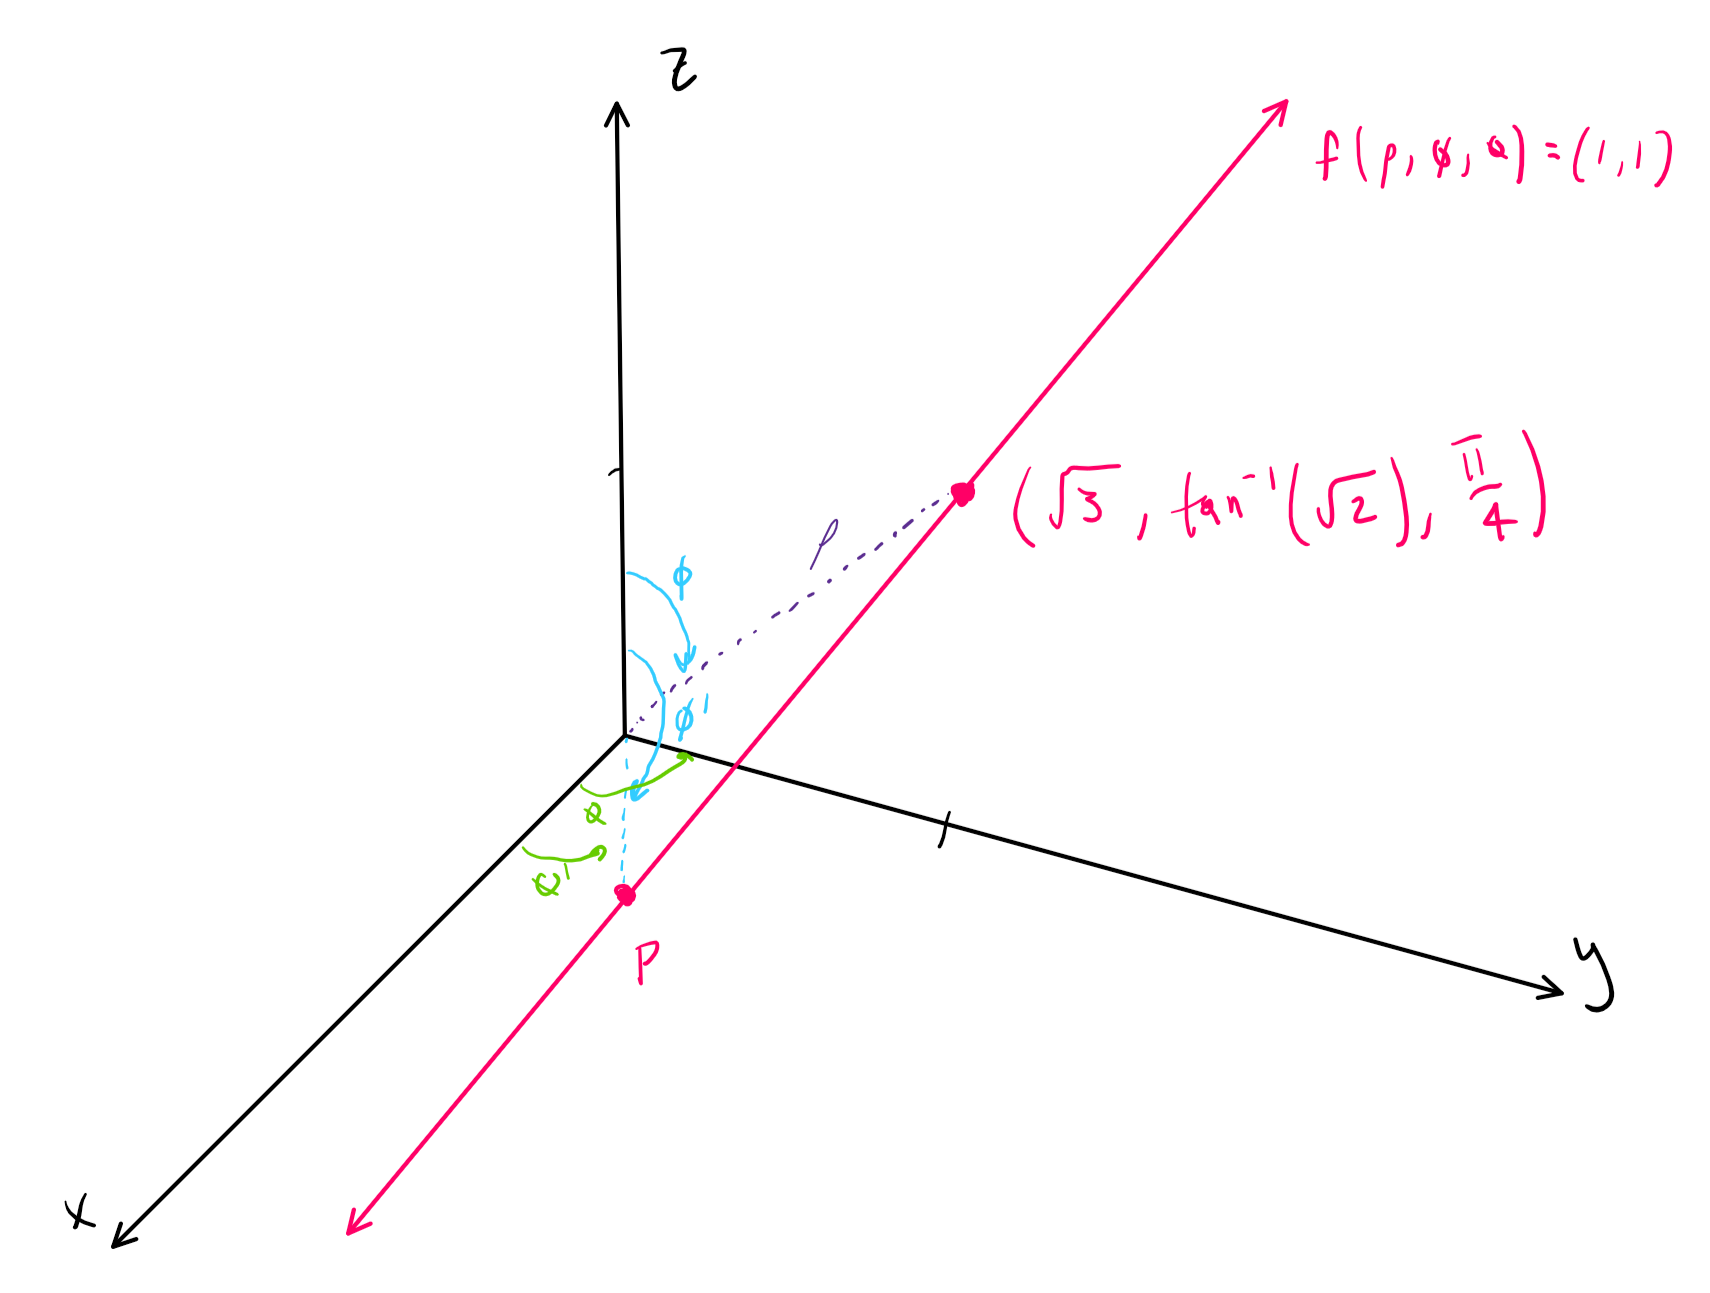
\includegraphics[scale=.5]{hw 6 (1).PNG}
    \end{center}
    
    Note, the point $P$ is after our change in $x$. So, $\phi'(\sqrt{3}) = \frac{\sqrt{6}}{6} > 0$ and $\theta'(\sqrt{3}) = -\frac{\sqrt{3}}{2} < 0$, which makes sense because when $\rho$ increases, then $\theta$ decreases and $\phi$ increases, which is what the math tells us.
\end{itemize}
\end{problem}


\begin{problem}{24}
Consider the equation $xe^y + ye^x = 0$. 

\begin{itemize}
    \item[(a)] Prove that this equation defines $y$ as a $C^\infty$ function of $x$ in a neighborhood of $(0,0)$.
    
    \begin{sol}
    Let $f : \mathbb{R}^2 \to \mathbb{R}$ be defined by $f(x,y) = xe^y + ye^x$. Then, $D_1f(x,y) = e^y + ye^x$, $D_{1,1}f(x,y) = ye^x$, $D_2f(x,y) = xe^y + e^x$, $D_{2,2}f(x,y) = xe^y$, and $D_{1,2}f(x,y) = e^y+e^x$.
    
    \vspace{1em}
    
    Let $P(n)$ be the statement "$\frac{\partial^n f}{\partial y^n}(x,y) = xe^y$".
    
    \underline{Base Case}: $\frac{\partial^2 f}{\partial y^2} = xe^y$. Thus, the base case is true. 
    
    \underline{Inductive Step}: Suppose $P(k)$ is true for some $k \geq 2$. Then, $\frac{\partial^k f}{\partial y^k}(x,y) = xe^y$, which implies $\frac{\partial^{k+1}f}{\partial y^{k+1}}(x,y) = xe^y$. So, $P(k+1)$ is true.
    
    \vspace{1em}
    
    Now, let $P(n)$ be the statement "$\frac{\partial^n f}{\partial x^n}(x,y) = ye^x$".
    
    \underline{Base Case}: $\frac{\partial^2 f}{\partial x^2}(x,y) = ye^x$. Thus, the base case is true. 
    
    \underline{Inductive Step}: Suppose $P(k)$ is true for some $k \geq 2$. Then, $\frac{\partial^k f}{\partial x^k}(x,y) = ye^x$, which implies $\frac{\partial^{k+1}f}{\partial x^{k+1}}(x,y) = ye^x$. So, $P(k+1)$ is true. Let $m \geq 2$ be arbitrary but fixed. Then, $\frac{\partial^m f}{\partial y^m}(x,y) = xe^y$ implies $\frac{\partial^{m+1} f}{\partial y^mx}(x,y) = e^y$. Also, $\frac{\partial^m f}{\partial x^m}(x,y) = ye^x$ implies $\frac{\partial^{m+1} f}{\partial x^my}(x,y) = e^x$. 
    
    \vspace{1em}
    
    Lastly, let $P(n)$ now be the statement "$\frac{\partial^{m+n} f}{\partial x^my^n}(x,y) = 0$. 
    
    \underline{Base Case}: $\frac{\partial^{m+1} f}{\partial x^my} = e^x$, which implies $\frac{\partial^{m+2} f}{\partial x^my^2}(x,y) = 0$. Thus, the base case is true. 
    
    \underline{Inductive Step}: Suppose $P(k)$ is true for some $k \geq 2$. Then, $\frac{\partial^{m + k} f}{\partial x^my^k}(x,y) = 0$, which implies $\frac{\partial^{m+k+1}f}{\partial x^my^{k+1}} = 0$. So, $P(k+1)$ is true.
    
    \hspace{1em} In total, we have $\frac{\partial f}{\partial x}(x,y) = e^y + ye^x$, $\frac{\partial f}{\partial y}(x,y) = xe^y + e^x$, $\frac{\partial^n f}{\partial x^n}(x,y) = ye^x$, $\frac{\partial^{n+1} f}{\partial x^n}(x,y) = e^x$, $\frac{\partial^n f}{\partial y^n}(x,y) = xe^y$, $\frac{\partial^{n+1} f}{\partial y^n}(x,y) = e^y$, and $\frac{\partial^{m+n} f}{\partial x^my^n}(x,y) = 0$ for all $n,m \geq 2$. Clearly, they are all continuous. Therefore, $f$ is $C^\infty$. Note, $f(0,0) = 0$ and $D_2f(0,0) = 1 \neq 0$, so by the implicit function theorem, there exists $r,s > 0$ and $g : B_s(0) \to B_r(0)$ defined by $f(x,g(x)) = 0$. Therefore, $f$ and $g$ are $C^\infty$ and $f(x,y) = 0$ defines $y$ as a $C^\infty$ function of $x$ in a neighborhood of $(0,0)$.
    \end{sol}
    
    \item[(b)] Let $y = g(x)$ be this implicitly defined function. Find $g'(0)$ and $g''(0)$.
    
    \begin{sol}
    Note, $$g'(x) = -\frac{D_1f}{D_2f} = -\frac{e^y+ye^x}{xe^y+e^x}$$ and 
    \begin{align*}
        g''(x) &= \frac{-(\frac{\partial f}{\partial y})^2\frac{\partial^2 f}{\partial x^2} + 2\frac{\partial f}{\partial x}\frac{\partial f}{\partial y}\frac{\partial^2 f}{\partial xy}-(\frac{\partial f}{\partial x})^2\frac{\partial^2 f}{\partial y^2}}{(\frac{\partial f}{\partial y})^3} \\ &= \frac{-(xe^y+e^x)^2(ye^x)+2(e^y+ye^x)(xe^y+e^x)(e^y+e^x)-(e^y+ye^x)^2(xe^y)}{(xe^y+e^x)^3}.
    \end{align*}
    So, from evaluating, we get $g'(0) = -1$ and $g''(0) = -4$.
    \end{sol}
    
    \item[(c)] Use this information to explain the appearance of the curve $xe^y + ye^x = 0$ near $(0,0)$.
    As $(x,y)$ approaches $(0,0)$, the slope is directed downward at a decreasing rate.
\end{itemize}
\end{problem}



%%%%%%%%%%%%%%%%%%%%%%%%%%%%%%%%%%%%%%%%
%Do not alter anything below this line.
\end{document}